\chapter{Color-Ordered Feynman Rules}
\label{sec:cofr}
\todo{figure out where this is appropriate to have (probably exactly here)}
In this appendix we list the color-truncated QCD Feynman rules, which can
for example be found in Ref.~\cite{Mangano1991}, in
Table \ref{tab:frqcd}. They are required for the calculation of
color-ordered amplitudes. We
assume all vertices are cyclically ordered and momenta are
outgoing. We use the light-cone decomposition for massive momenta
\begin{align}
p &=  p^\flat + \frac{m^2}{2p\cdot q}q,&  q^2& =0,
\end{align}
with an arbitrary $p\cdot q\neq 0$ light-like reference momentum $q$
and use the spinor-helicity formalism, as for example presented in Ref.~\cite{Dixon:1996wi,DittmaierWeyl}. Furthermore, we list the Feynman rule
for the \ew~vertex used
in this thesis in Table \ref{tab:frew}. The full set of SM Feynman rules can for
example be found in Ref.~\cite{Bohm:2001yx,Schwartz:2013pla}.



\begin{table}[]
\centering
\caption{Feynman rule for the \ew~vertex used in
  this work with outgoing momenta, adapted from Ref.~\cite{Bohm:2001yx}. $V_{ij}$ denote entries of the CKM matrix.}
\label{tab:frew}
\begin{tabular}{l}
\begin{tabularx}{\textwidth}{cl}
    \hline\hline
    \noalign{\vskip 2.5mm}
    \textbf{Electroweak Vertex}\\
    \noalign{\vskip 2mm}
    \hline
    \noalign{\vskip 4mm}
\raisebox{-.4\height}{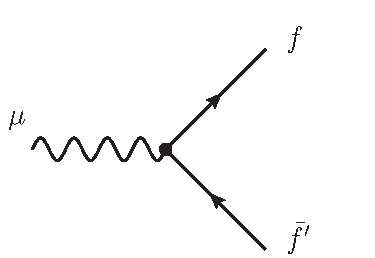
\includegraphics[clip,width=0.28\textwidth]{figures/qqv}}
&$\displaystyle = i e \gamma^\mu \left(C_{L}\frac{1-\g5}{2}
   + C_{R}\frac{1+\g5}{2}\right) $\\
    \noalign{\vskip 4mm}
    \hline
    \noalign{\vskip 8mm}
\multicolumn{2}{c}{
\begin{tabular}{ccccccc}
$V f \bar{f}^\prime$ & $\gamma f_i \bar{f}_j $& $Z f_i \bar{f}_j $&
$W^+ u_i \bar{d}_j  $& $W^- d_j \bar{u}_i $& $W^+ \nu_i \bar{l}_j $& $W^- l_j \bar{\nu}_i$\\
    \noalign{\vskip 2mm}
    \hline
    \noalign{\vskip 2mm}
$C_L$  & $\displaystyle -Q_f \delta_{ij}$ & $\displaystyle g_f^-
\delta_{ij}$ & $\displaystyle\frac{1}{\sqrt{2}{s_w}}V_{ij}$
& $\displaystyle\frac{1}{\sqrt{2}{s_w}}V_{ji}^*$  &
$\displaystyle\frac{1}{\sqrt{2}{s_w}}\delta_{ij}$ &$\displaystyle\frac{1}{\sqrt{2}s_w}\delta_{ji}$ \\
    \noalign{\vskip 2mm}
$C_R$ & $\displaystyle -Q_f \delta_{ij}$ & $\displaystyle g_f^+ \delta_{ij}$ &$0$ &$0$&$0$&$0$\\
\end{tabular}}\\
    \noalign{\vskip 8mm}
    \hline
    \noalign{\vskip 8mm}
\multicolumn{2}{c}{where \hspace{0.8cm}$\displaystyle g_f^+ = -\frac{s_w}{c_w}Q_f,$ \hspace{0.8cm}$\displaystyle g_f^- = \frac{I_{W,f}^3-s_w^2Q_f}{s_wc_w},$\hspace{0.8cm}$s_w=\sin(\theta_W),$\hspace{0.8cm}$c_w=\cos(\theta_W)$.}\\
    \noalign{\vskip 4mm}    
\hline\hline
\end{tabularx}
\end{tabular}
\end{table}



\begin{table}[]
\centering
\caption{Color-truncated QCD Feynman rules in Feynman gauge.}
\label{tab:frqcd}
\begin{tabular}{l}
\begin{tabularx}{\textwidth}{ll}
    \hline\hline
    \noalign{\vskip 2.5mm}
    \textbf{Propagators}\\
    \noalign{\vskip 2mm}
    \hline
    \noalign{\vskip 4mm}
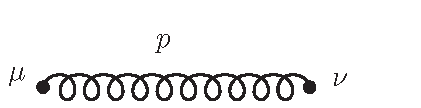
\includegraphics[clip,width=0.2\textwidth]{figures/gp2}
&$\displaystyle = \frac{-ig^{\mu\nu}}{p^2}$\\
    \noalign{\vskip 2mm}

\includegraphics[clip,width=0.15\textwidth]{figures/qp2} &
$\displaystyle  = \frac{i(\slashed{p}+m)}{p^2-m^2}$\\
    \noalign{\vskip 2.5mm}
    \hline
    \noalign{\vskip 2.5mm}
    \textbf{Vertices}\\
    \noalign{\vskip 2mm}
    \hline
    \noalign{\vskip 4mm}
\raisebox{-.4\height}{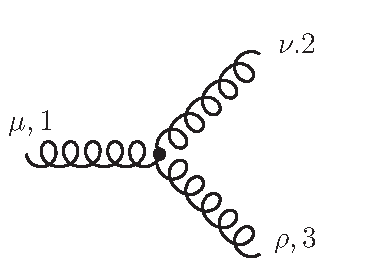
\includegraphics[clip,width=0.2\textwidth]{figures/gggv}}
& $\displaystyle = \frac{i}{\sqrt{2}} \left[
        g^{\mu\nu}(p_1-p_2)^\rho+g^{\nu\rho}(p_2-p_3)^\mu+g^{\rho\mu}(p_3-p_1)^\nu\right]$\\
\raisebox{-.4\height}{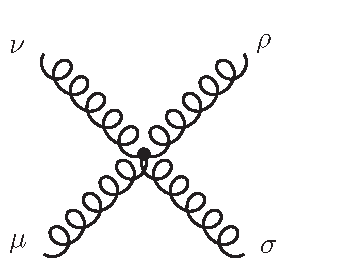
\includegraphics[clip,width=0.2\textwidth]{figures/gggg}}
&  $\displaystyle= i \left[ g^{\mu\rho}g^{\nu
        \sigma}-\frac{1}{2}(g^{\mu\nu}g^{\rho\sigma}+g^{\mu\sigma}g^{\nu\rho})\right]$ 
\end{tabularx}\\
    \noalign{\vskip 2mm}
\begin{tabularx}{\textwidth}{lp{4.5cm}ll}
\raisebox{-.4\height}{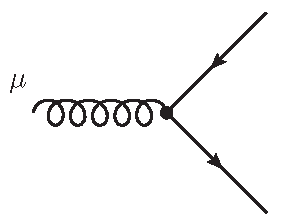
\includegraphics[clip,width=0.15\textwidth]{figures/qqg}}
&
$\displaystyle= \frac{i}{\sqrt{2}} g_{s} \gamma^{\mu}$&
\raisebox{-.4\height}{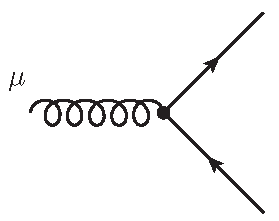
\includegraphics[clip,width=0.15\textwidth]{figures/qqg2}}
&
 $ \displaystyle=  -\frac{i}{\sqrt{2}} g_{s} \gamma^{\mu}$\\
\end{tabularx}\\
\begin{tabularx}{\textwidth}{p{2cm}lp{2cm}l}
    \noalign{\vskip 2.5mm}
    \hline
    \noalign{\vskip 2.5mm}
    \multicolumn{2}{l}{\textbf{Outgoing Fields}}\\
    \noalign{\vskip 2mm}
    \hline
    \noalign{\vskip 4mm}
%ubar
{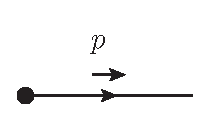
\includegraphics[clip,width=0.15\textwidth]{figures/wfq}}
&
\begin{tabular}{ll}
\ldelim\{{3}{4mm}&$\displaystyle \bar{u}_+ =  [ p^\flat|+
\frac{m}{\langle q p^\flat\rangle} \langle q|$\\
    \noalign{\vskip 2mm}
&$\displaystyle  \bar{u}_-=\langle p^\flat|+\frac{m}{[q p^\flat]} [q|$
\end{tabular}&
%epsilon*
{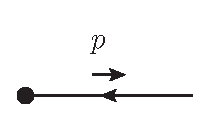
\includegraphics[clip,width=0.15\textwidth]{figures/wfqb}}
& 
\begin{tabular}{ll}
\ldelim\{{3}{4mm}&$\displaystyle v_+ =
|p^\flat]-\frac{m}{\langle{p^\flat} q\rangle}\ket{q}$\\
    \noalign{\vskip 2mm}
&$\displaystyle  v_-= |p^\flat\rangle-\frac{m}{[p^\flat q]}|q]$
\end{tabular}\\
    \noalign{\vskip 4mm}   
%v
{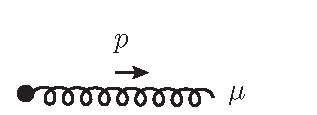
\includegraphics[clip,width=0.20\textwidth]{figures/wfg}}
& 
\begin{tabular}{ll}
\ldelim\{{3}{4mm}&$\displaystyle \epsilon^*_+ =\frac{[q |\gamma^\mu|p\rangle}{\sqrt{2}[pq]} $\\
    \noalign{\vskip 2mm}
&$\displaystyle  \epsilon^*_-=\frac{\langle q |\gamma^\mu|p]}{\sqrt{2}\langle q
  p \rangle}$
\end{tabular}\\
    \noalign{\vskip 2mm}    
\hline\hline
\end{tabularx}
\end{tabular}
\end{table}





%\chapter{Results for Selected Scalar Integrals}
%\label{sec:massivebasisint}
%Among the additional scalar integrals appearing in the master
%integral decomposition in Section \ref{sec:scmi} for processes involving massive quarks are the
%tadpole integral $I_1(m^2)$ and the bubble integral with a single massive leg in
%one corner $I_2(m^2;0,m^2)$. For vanishing masses, both
%integrals are scaleless and vanish in dimensional regularization. They
%are given in dimensional regularization with $D=4-2\epsilon$ by
%\begin{align}\label{eq:tadint}
%I_1(m^2) \equiv I_{1}=\frac{\mu_R^{2\epsilon}}{ic_{\Gamma}}\int
  %\frac{\dd[D]{\ell}}{(2\pi)^D}\frac{1}{(\ell^2-m^2)} =
   %m^2\left(\frac{1}{\epsilon}+\log(\frac{\mu_R^2}{m^2})+1 \right)+\mathcal{O}(\epsilon),
%\end{align}
%and
%\begin{align}\label{eq:olbmint}
%I_2(m^2;0,m^2) \equiv
%I_{2,m^2}=\frac{\mu_R^{2\epsilon}}{ic_{\Gamma}} \int
  %\frac{\dd[D]{\ell}}{(2\pi)^D}\frac{1}{\ell^2((\ell-p)^2-m^2)} =
  %\left(\frac{1}{\epsilon}+\log(\frac{\mu_R^2}{m^2})+2 \right)+\mathcal{O}(\epsilon),
%\end{align}
%where the small imaginary part $i\epsilon$ in the inverse propagators
%is understood implicitly as $D_i=(\ell_i^2-m_i^2+i\epsilon)$ and $c_\Gamma=(4\pi)^{-(2-\epsilon)}\Gamma^2(1-\epsilon)\Gamma(1+\epsilon)/\Gamma(1-2\epsilon)$. The integrals are taken from Ref.~\cite{Ellis:2007qk}.





%\chapter{Tadpole Coefficients From UV matching}
%\label{sec:uvmatch}
%In an application of numerical unitarity to processes with a single mass circulating in
%the loop, one can avoid the computation of single cuts in order to extract the
%tadpole coefficient.\footnote{For more complex processes with different masses
%in the loop one has several tadpole coefficients.} Instead, as
%proposed in Ref.~\cite{Bern:1995db,Badger2008}, one can match the known $UV$
%singularity structure of the mass-renormalized amplitude \cite{Catani:2000ef} to the $UV$ poles of tadpole, bubble and renormalization contributions. The
%$UV$-divergent part of the tadpole integral and bubble integrals are
%given in Eq.~\eqref{eq:tadint} and Eq.~\eqref{eq:olbmint} of Appendix \ref{sec:massivebasisint} by
%\begin{align}
 %I_{1\rvert_{\frac{1}{\epsilon}}} &= \tilde{I}_1 = m^2 &
 %I_{2,i\rvert_{\frac{1}{\epsilon}}} &= \tilde{I}_{2,i} = 1  
%\end{align}
%for all $i$ and are in particular independent of other kinematical
%invariants. Since tadpole and bubble integrals as well as mass renormalization counterterms are the only sources of $UV$ divergencies for
%mass-renormalized one-loop
%amplitudes, one can deduce the tadpole coefficient by matching the known
%$UV$-pole structure of each primitive amplitude \cite{Catani:2000ef} to the $UV$-poles of the
%combined bubble, tadpole and renormalization contributions
%\begin{align}
  %\begin{split}
  %\mathcal{A}_{\rvert_\text{UV}}^{\text{mass ren.}} & =  \sum_i b^0_i
  %\tilde{I}_{2,i}+a^0 \tilde{I}_1 + \alpha_{\text{mass ren.}}\\
%&\Rightarrow   a^0 =  \frac{1}{m^2}\left(\mathcal{A}_{\rvert_\text{UV}}^{\text{mass ren.}} -  \sum_i
%b^0_i  -\alpha_{\text{mass ren.}}\right) ,
  %\end{split}
%\end{align}
%with the mass renormalization contribution $\alpha_{\text{mass ren.}}$. In practice, this implies extracting the $UV$ pole structure
%of primitive amplitudes from that of the full amplitude
%\cite{Catani:2000ef} as laid
%out in Ref.~\cite{Ellis:2011cr}. In the work presented in this thesis we do
%not apply this technique but follow the straightforward application of numerical unitarity
%and compute single cuts explicitely. In particular since this is
%independent of the number of masses in the loop.





\chapter{Operations on \texorpdfstring{$\gamma$}{Gamma} Matrices}\label{sec:identities}


In the following we derive the values of the contraction of the
tensors $w_0$ and $v_n$ which are used in 
eqs.~\eqref{eq:decompqqbar} and \eqref{eqn:4qampltensor}.
%
In this appendix we take $d$ to be an even integer denoting the
dimension of the space for which the Clifford algebra is defined
and we denote the dimension of the $\gamma$-matrix
representation by
$d_t=\Tr(\mathbb{1}_{[d]})=2^{d/2}$.
In the main text, we are interested in the case
%
\begin{eqnarray}
  d = (D_s-4)\,.
\end{eqnarray}
%
Since amplitude computations are homogeneous in the
factor $d_t$, it can be factored out and replaced by 
a suitable value in order to suit the four-dimensional 
limit. In this appendix, we keep the parameter $d_t$ in analytic
form in order to maintain a consistent finite-dimensional
algebra and for clarity of the equations. 
In the main text we use formulas with the replacement
$d_t\rightarrow 1$ imposed, which is the value consistent with a
calculation in dimensional regularization \cite{Collins:1984xc}.

We start with the trivial case of $w_0$ which appears in 
eq.~\eqref{eq:decompqqbar}. It is easy to find that
%
\begin{eqnarray}
  w_0=\delta_\kappa^\lambda\,,\qquad 
  w^0=\delta^\kappa_\lambda/d_t\,,\qquad 
  w_0\cdot w^0=\delta_\kappa^\lambda  \delta^\kappa_\lambda/d_t=1\,.
\end{eqnarray}

For the tensors $v_n$ of eq.~\eqref{eqn:4qampltensor} we
must first consider traces of $\gamma$-matrix chains of
the form
%
\begin{align}\label{eq:basisGammaChainII}
\gamma_{[d]}^{\mu_1 \ldots \mu_n} = \frac{1}{n!} \sum_{ \sigma\in
S_n} \sgn(\sigma) \gamma_{[d]}^{\mu_{\sigma(1)}} \ldots
\gamma_{[d]}^{\mu_{\sigma_n}}\,,
\end{align}
with $S_n$ denoting the set of permutations of $n$
integers and $\sgn(\sigma)$ the signature of the permutation $\sigma\in S_n$.
%
Given a unitary
representation of the $\gamma_{[d]}^\mu$ matrices, hermitian
conjugation reverses the $\gamma$-matrix chains and flips the
Lorentz index position.
%
This can be seen from the definition of the Clifford algebra
(\cref{eqn:defClifford}) which implies 
$\gamma_{[d]}^\mu \gamma^{}_{[d]\mu} = \mathbb{1}_{[d]}$ for 
any fixed~$\mu$.
Assuming that the $\gamma_{[d]}^\mu$ are unitary, i.e.
$(\gamma_{[d]}^\mu)^\dagger = (\gamma_{[d]}^\mu)^{-1}$,
then implies
$(\gamma_{[d]}^\mu)^\dagger=\gamma_{[d]\mu}$. 
For the above product of $\gamma$ matrices this in turn leads to
%
\begin{eqnarray}
  (\gamma_{[d]}^{\mu_1 \ldots \mu_n} )^\dagger =\,
  \gamma_{[d]\mu_n \ldots \mu_1}^{\phantom{\mu}} \,.
\end{eqnarray}
%
%
Unitary representations for the Clifford algebra can always be
found as explained for example in 
ref.~\cite{Kreuzer:susylectures}.
%
We will require the following traces of antisymmetric
$\gamma$-matrix chains,
%
\begin{eqnarray}
  \label{eq:traceChain}
  \Tr(\gamma_{[d]}^{\mu_1 \ldots \mu_n} \gamma^{
    \phantom{\mu}}_{[d]\,\nu_m \ldots \nu_1})= 
    \left\{ \begin{array}{cc} d_t 
      \sum_{ \sigma\in  S_n} \sgn(\sigma)
      \delta^{\mu_{\sigma(1)}}_{\nu_1}\cdots\delta^{\mu_{\sigma(n)}}_
      {\nu_n} &\qquad m=n   \\
      0 &\qquad m\neq n\end{array}  
    \right. 
    \,,
  \end{eqnarray}
%
where the summation runs over all permutations $S_n$ of $n$ elements.
The traces are computed in fixed integer dimensions where the dimensions of the
$\gamma$-matrix representation is taken to be $d_t$ dimensional.
For contracted Lorentz indices we will also use that
\begin{eqnarray}
  \label{eqn:simpletrace}
  \sum_{\mu_1,\ldots,\mu_n} 
  \sum_{ \sigma\in  S_n} \sgn(\sigma)
  \delta^{\mu_{\sigma(1)}}_{\mu_1}\ldots
  \delta^{\mu_{\sigma(n)}}_{\mu_n}
  = \frac{d!}{(d-n)! }\,.
\end{eqnarray}
The sum counts the number of antisymmetric tensors of
rank $n$ in $d$ dimensions, which is the number of ways to 
choose an ordered subset of $n$ elements from a fixed set of $d$
elements.
%
With these preparatory equations we can
compute the inner products of the $v_n$ tensors of 
\cref{eqn:4qtensors}
which yield the normalisation factors $c_n$
of \cref{eqn:vnproducts}:
\begin{align}
  \begin{split}
    \label{eq:cnCalc}
    c_n=v_n^\dagger\cdot v_n =&\,
%
    \Tr(\gamma_{[d]\,\mu_n \ldots \mu_1} \gamma_{[d]}^
    {\nu_1 \ldots \nu_n}) \,
%
    \Tr(\gamma_{[d]}^{\mu_n \ldots \mu_1} \gamma_{
    [d]\,\nu_1 \ldots \nu_n}) \\
    =&\,
    d_t^2 \sum_{\sigma\in  S_n} 
    \sum_{\mu_1,\ldots,\mu_n}
    \sum_{\tilde \sigma\in S_n}
    \sum_{\nu_1,\ldots,\nu_n}
%
    \sgn(\sigma)
    \sgn(\tilde\sigma)
    \delta^{\mu_{\sigma(n)}}_{\nu_1}\cdots\delta^{\mu_{\sigma(1)}}_{\nu_n}
    \delta_{\mu_{\tilde\sigma(n)}}^{\nu_1}\cdots
    \delta_{\mu_{\tilde\sigma(1)}}^{\nu_n}
    \\
%
    =&\,d_t^2 \sum_{\sigma\in  S_n} 
    \sgn(\sigma)
    \left(
    \sum_{\mu_1,\ldots,\mu_n}\sum_{\tilde \sigma\in S_n}
%
    \sgn(\tilde\sigma)
    \delta^{\mu_{\sigma(n)}}_{\mu_{\tilde\sigma(n)}}
    \cdots
    \delta^{\mu_{\sigma(1)}}_{\mu_{\tilde\sigma(1)}}
    \right)
    \\
%
    =&\, d_t^2 \sum_{\sigma\in  S_n} 
    \sgn(\sigma)^2 \frac{d!}{(d-n)!}\\
    =&\, d_t^2 \frac{d!\,n!}{(d-n)!}\,.
  \end{split}
\end{align}
In the above formulas the summation over the indices $\nu_i$ is 
trivially performed. In the next step, we isolate a contribution
of the form that we computed in eq.~\eqref{eqn:simpletrace},
which gives the same result for each permutation $\sigma$ but
multiplied by $\sgn(\sigma)$. The final results follows
trivially.
As expected, for each $n$ the result has zeros in the dimensions
$d$ for which there are insufficient distinct labels 
$\mu_i$ and $\nu_i$ available to form antisymmetric index 
configurations of $n$ indices.
We recall that in the main text we set $d_t=1$ and $d=D_s-4$.


Finally we collect the results for the contractions of the 
tensor $\tilde v_m$ and $v_n$ required for amplitudes with two
quark lines of identical flavor,
see \cref{eq:basisIdentical}.
These contractions lead to a single trace instead of a product 
of traces as was the case in eq.~\eqref{eq:cnCalc}.
We refer to the above intuitive argument: tensor 
contractions including $v_n$ or $\tilde v_n$ vanish 
whenever the dimensionality $d$ is insufficient to accommodate
the respective antisymmetric index arrangements in the Lorentz 
indices $\mu_i$ and $\nu_i$.
In particular this implies that contractions including the
tensors $v_{n}$ are proportional to $d$ for $n\neq0$. We find
that 
\begin{align}
  \begin{split}
    \tilde v_0^\dagger \cdot v_0 &=
    \delta^{\kappa_1}_{\lambda_2} \delta^{\kappa_2}_{\lambda_1}
    \delta_{\kappa_1}^{\lambda_1} \delta_{\kappa_2}^{\lambda_2} 
    = d_t \,, \\
    \tilde v_m^\dagger \cdot v_{n} &=d_t\,d\,p_{mn}(d) = 
    {\cal O}(\epsilon)\,,\qquad\textrm{for }\{m,n\}\neq\{0,0\}\,.
  \end{split}
\end{align}
Here $p_{mn}(d)$ is a polynomial-valued matrix which we 
will not require explicitly for the present paper, and in the
last equality we made explicit the fact that in this paper we 
are interested in the case $d=D_s-4={\cal O}(\epsilon)$.



\chapter{Numerical Algorithms}

\section{Finite Fields and Floating Point Arithmetics}

Definition of finite fields.

Brief comparisong of finite fields vs floating point.

usage of finite fields in \cite{Klappert:2019emp,Peraro:2016wsq,Peraro:2019svx}

\subsection{Rational Reconstruction}
\begin{figure}[ht]
  \begin{center}
    \begin{tikzpicture}[auto, node distance = 3cm,shorten >= 2pt]
      \node [rectangle, draw, text centered] (x) {$\mathbf{x}$};

      \node [above right = 0.3cm and 0.7cm of x] (xmod1) {$\mathbf{x}\mod p_1$};
      \node [right  of=xmod1] (cmod1) {$c\mod p_1$};

      \node [below right = 0.3cm and 0.7cm of x] (xmodn) {$\mathbf{x}\mod p_n$};
      \node [right  of=xmodn] (cmodn) {$c\mod p_n$};


      \node [below = 0cm of xmod1] () {$\vdots$};
      \node [below = 0cm of cmod1] () {$\vdots$};
      \node [below right = 0cm and 0.1cm of xmod1] () {$\vdots$};

      \node [ellipse, draw, text centered, right =6cm of x, node distance = 3cm, text width = 1.5cm, inner sep = 1pt] (crt) {\baselineskip=-10pt \tiny Chinese Remainder Theorem \par};
      \node [right = 0.5cm of crt] (cmodP) {\minibox{ $c\mod P$  \\ \footnotesize $\left(P\equiv\prod_i p_i\right)$} };

      \node [rectangle, draw, text centered, right of=cmodP, node distance = 3cm] (c) {$c$};


      \path [line,->] (x) -- (xmod1.west);
      \path [line,->] (x) -- (xmodn.west);

      \path [line,->] (xmod1.east) -- node [above]{$f$} (cmod1.west);
      \path [line,->] (xmodn.east) -- node [above]{$f$} (cmodn.west);

      \path [line,->] (cmod1.east) -- (crt);
      \path [line,->] (cmodn.east) -- (crt);

      \path [line,->] (crt) -- (cmodP);

      \path [line,->] (cmodP) -- node [above]{\small $n,d < \sqrt{P}$} (c);
    \end{tikzpicture}
  \end{center}
  \caption{The diagram representing rational reconstruction.}
  \label{fig:RatReconstr}
\end{figure}

\section{Solving Linear Systems of Equations}
For floating numerical stability is important.

For finite fields only field operations. PLU decomposition algorithm.

Put the one-loop cases here? Fourier transform and hard-coded solutions for inversions?

\section{On-Shell Loop Momenta and Finite Fields}
The extension of unitarity approaches to employ only operations
defined in an algebraic field was proposed 
in ref.~\cite{Peraro:2016wsq}.
A finite-field based calculation allows to compute exact values
for the integral coefficients $c_{\Gamma,i}$ of eq.~\eqref{eq:A}
in a numerical framework.
This idea
was applied recently in \cite{Badger:2017jhb,Abreu:2017hqn} for
pure gluon-scattering amplitudes, and here we discuss our
implementation for amplitude computations with fermions.

\subsubsection{Generic Algebraic Extension}

From here on we denote by $\mathbb{F}$ an arbitrary 
number field. In practice, we will be interested in
$\mathbb{F}$ being the field of rational numbers $\mathbb{Q}$
or the finite field $\mathbb{Z}_p$
of all integers modulo a prime number $p$.
In general, polynomial equations do not have solutions in 
$\mathbb{F}$. This is at odds with the fact that
in a unitarity-based approach one needs 
to generate loop momenta which satisfy a set of quadratic
conditions corresponding to setting propagators to zero.
%
In the presence of fermions, the situation becomes more 
complicated due to the extension of the Clifford algebra beyond 
four dimensions. More specifically, terms such as $\ell^\mu
\gamma_{[D_s]\mu}$ exhibit the $(D-4)$-dimensional
components of the loop momenta,
which are in general not 
$\mathbb{F}$-valued for on-shell momenta
(more concretely, if we work on the field of rational numbers
these components are in general irrational),
leading to terms in the sub-currents of the
Berends-Giele recursion that are not $\mathbb{F}$-valued. 
%
To address this issue,
we start with a parametrization of the on-shell spaces as in 
ref.~\cite{Abreu:2017hqn} but always use normalized basis
vectors. We write the two-loop momenta as
\begin{equation}
    \ell_1 = (\ell_{1,[4]}, \vec{\mu}_1)\,,\quad \quad \quad
    \ell_2 = (\ell_{2,[4]}, \vec{\mu}_2)\,, 
    \label{eq:loopmomenta}
\end{equation}
where we denote their $(D-4)$-dimensional components as 
$\vec{\mu}_1$ and $\vec{\mu}_2$. Next, we choose an orthonormal
basis $\vec{n}_i$ of the $(D-4)$-dimensional space with
$n_1$ in the direction of $\vec{\mu}_1$ and write
\begin{equation}
\vec{\mu}_1 = r_1 \vec{n}_1, \quad  \vec{\mu}_2 = \frac{\mu_{12}}{\mu_{11}} r_1 \vec{n}_1 + r_2 \vec{n}_2
  \quad \mathrm{where} \quad r_1 = \sqrt{\mu_{11}}, \quad r_2 = 
  \sqrt{\mu_{22} - \mu_{12}^2/\mu_{11}},
\end{equation}
with $\mu_{ij}=\vec{\mu}_i\cdot\vec{\mu}_j$.
In a theory containing only vector particles we only ever need 
the values $r_i^2$, which are $\mathbb{F}$-valued both on- and
off-shell \cite{Abreu:2017hqn}. In contrast, in a theory with
fermions, components of Berends-Giele currents will take the
generic form
\begin{equation}
  \label{eq:ExtendedAlgebra}
  a_{00} + a_{10} r_1 + a_{01} r_2 + a_{11} r_1 r_2, 
\end{equation}
which is not $\mathbb{F}$-valued.
In order to nevertheless be able to
work in the field $\mathbb{F}$,
we consider 
the algebra $\mathbb{V}$ over the field $\mathbb{F}$, with 
$\mathbb{V}$ the vector space spanned by the basis 
$\{r_0=1,r_1,r_2,r_1r_2\}$ and equipped with the standard
addition and multiplication.
All components of the Berends-Giele are elements 
in the algebra, and can thus be written as a linear combination
of the $r_i$ with $\mathbb{F}$-valued coefficients. More
concretely, this means we only need to determine the $a_{ij}$ 
in eq.~\eqref{eq:ExtendedAlgebra} which are $\mathbb{F}$-valued
by construction.

An important observation is that, although the coefficients 
$a_{10}$, $a_{01}$ and $a_{11}$ in 
eq.~\eqref{eq:ExtendedAlgebra} are non-zero in
intermediate stages of the calculations, they vanish
for the integrands of helicity amplitudes as defined in 
eq.~\eqref{eq:tensorDecomposition}. This cancellation of the
$r_i$ terms holds in the HV scheme and
is due to the projection onto the invariant tensors 
$v_n$ of eq.~\eqref{eq:tensorDecomposition}, 
which yields polynomials in the Lorentz invariants 
$\mu_{ij}$ at the integrand level
(see the discussion in section \ref{sec:ParamIntegrands}).


\subsubsection{Only Vector Particles}
%
In ref.~\cite{Abreu:2017hqn}, this was resolved
by making sure that all scalar products
between the momenta in the problem were $\mathbb{F}$-valued.


\subsubsection{Special Metric Signature}

Any Lorentz-invariant quantity such as helicity amplitudes (normalized by an appropriate spinor weight)
depends on the space-time metric tensor only through contractions with momenta and states of external particles.
Thus  without loss of generality we can choose to use an alternating metric signature $(+,-,+,-,\ldots)$
and modify external momenta such that all Lorentz invariants remain unchanged.

We then can parametrize the two-dimensional loop-momentum components
$\vec{\mu}_1$ and $\vec{\mu}_2$ as follows:
\begin{equation}
  \vec{\mu}_1(t)  = \frac{1}{2}\begin{pmatrix}
    t+\dfrac{\mu_{11}}{t} \\
    t-\dfrac{\mu_{11}}{t} \\
  \end{pmatrix}, \quad
  \vec{\mu}_2(t)  = \frac{\mu_{12}}{\mu_{11}}\vec{\mu}_1(t) - \frac{r}{\mu_{11}}~\frac{1}{2}\begin{pmatrix}
    t-\dfrac{\mu_{11}}{t} \\
    t+\dfrac{\mu_{11}}{t} \\
  \end{pmatrix},
  \label{eq:muparam}
\end{equation}
where $t$ is a free dimensionful parameter that leaves the scalar products
$r = \sqrt{\mu_{12}^2-\mu_{11} \mu_{22}}$ and 
$\mu_{ij} = \mu_i^1 \mu_j^1 - \mu_i^2 \mu_j^2$ invariant. %

This parametrization allows to reduce the size of the algebraic extension $\mathbb{V}$ generated by \cref{eq:ExtendedAlgebra},
which is a significant optimization of numerical evaluations.


\todo{Note on other possibilities to avoid solving on-shell conditions.}


\section{Exact Interpolation of Functions over Finite Fields}
\subsection{Univariate Polynomials}
\subsection{Multivariate Polynomials}




\chapter{Spinor-Helicity}
\label{chap:4dspinhel}

here describe four-dimensional spinor-helicity

\todo{denormalized spinors for finite fields}



\chapter{van Neerven-Vermaseren Basis}
In the van Neerven-Vermaseren (NV) construction
\cite{Neerven1984a}, the $D$-dimensional
space-time is decomposed into a physical space and its complement, the
transverse space. The NV construction is used for integrand
parameterizations \cite{Ellis:2007br,Ita:2011hi}. Consider $r$ inflow momenta $p_1,\dots,p_r$. The
physical space is then spanned by these $r$ momenta and has dimensions
$D_p=\min(D,r-1)$, since the $r$ momenta are in general linearly dependent and one degree of freedom is absorbed by momentum
conservation $\sum_{i=1}^rp_i = 0$. Whenever $r>D$, one can find
additional relations to reduce the higher point scalar integrals to
lower point ones \cite{Melrose1965}. For example, if $D=4$, one finds
a basis with a maximal rank of $4$. The physical space therefore forms
a lower dimensional subspace whenever $r\leq D$. The complent to the
physical space is called
transverse space and has dimension $D_t=\max(0,D-r+1)$, such that
\begin{align}
  D=D_p+D_t.
\end{align}
We assume that the momenta $p_1,\dots,p_r$ are ordered, such that the
first $D_p$ vectors are linearly independent. The corresponding dual
vectors are called $v_{1},\dots,v_{D_p}$. The transverse basis
vectors are denoted $n_{1},\dots,n_{D_t}$ and we have the following properties
\begin{align}
    n_i\cdot n_j &= \delta_{ij}, & n_i\cdot p_j &= 0,\\
   v_j \cdot n_i  &= 0, & v_j\cdot p_i &= \delta_{ij}.\notag
\end{align}
For the case that $r > D$, the space
is parameterized solely in terms of linearly independent vectors
$p_i$. 
 The metric tensor is thus decomposed in the NV basis as 
\begin{align}
  g^{\mu\nu} = \sum_{i=1}^{D_p}p_i^\mu v_i^\nu+\sum_{i=1}^{D_t}n_i^\mu n_i^\nu,
\end{align}
with the projector into the transverse space consquently given by
\begin{align}\label{eq:metricpron}
  (g_\perp)^{\mu\nu} \equiv  \sum_{i=1}^{D_t}n_i^\mu n_i^\nu = g^{\mu\nu}- \sum_{i=1}^{D_p}p_i^\mu v_i^\nu.
\end{align}
One can thus decompose the loop momentum in the NV basis as 
\begin{align}
  \ell^\mu = \sum_{i=1}^{D_p}(\ell\cdot p_i)
  v_i^\mu+\sum_{i=1}^{D_t}(\ell\cdot n_i) n_i^\mu,
\end{align}
with the projections of the loop momentum on the transverse space
$t_i(\ell) = (\ell \cdot n_i)$.  In actual computations with $D>4$, only a specific combination of the
projection on the transverse space is relevant. Since external
particles remain in $4$-dimensions, the additional components of the
loop momentum are only relevant in contractions of the loop momentum
with itself
\begin{align}
  \mu^2 = -\ell_{[D-4]}^2 \equiv \sum_{i=5}^D(\ell \cdot n_i)^2,
\end{align}
for explicit integer $D$-dimensions. Only this combination is of
relevance in $D\neq 4$-dimensional calculations. The $n_{i>4}$ are the transverse
vectors of the $D-4$-dimensional space. One can split up the
decomposition into a $4$-dimensional part and a $D-4$-dimensional part
and gets for the projector into the transverse space
\begin{align}\label{eq:metricprond}
\begin{split}
  (g_\perp)^{\mu\nu} &=  \sum_{i=1}^{D_t}n_i^\mu n_i^\nu=\sum_{i=1}^{4-r+1}n_i^\mu n_i^\nu +  \sum_{i=5}^{d}n_i^\mu n_i^\nu.
\end{split}
\end{align}



\chapter{Twistor Parametrization}
\todo{twistor parametrization} 
see e.g. Bobadilla thesis
